\chapter{Advanced Architectures}\label{sec:advanced_architectures}

\section{Convolutional Nets}

A convolutional neural net (CNN), seen in Figure~\ref{fig:CNN_architecture}, mimics the neural architecture seen in the visual cortex of animals. In fact, CNN simulations compared against neural imaging results in the visual pathways of salamanders and cats have yielded remarkably good results, showing that the CNN is a good descriptor of the kind of processing that actually happens in a living brain.

\begin{figure}[htbp]
    \centering
    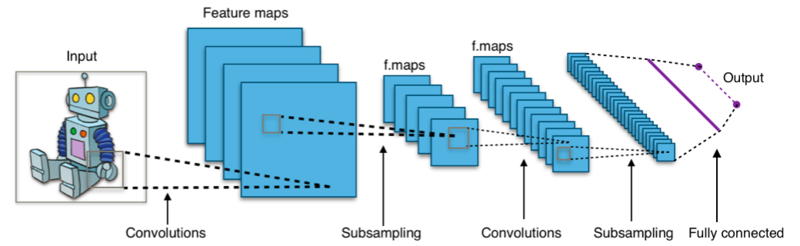
\includegraphics[width=\linewidth]{Images/ML/CNN_architecture.png}
    \caption{The structure of a typical CNN, taken from~\cite{CNN_architecture}. The alternating use of convolutional and downsampling layers is typical, as is the use of unfolding, concatenation, and a final fully connected layer at the end.}
    \label{fig:CNN_architecture}
\end{figure}

A CNN works by exploiting pattern finding filters at multiple scales. That is, first we look at small regions on an image, and look for simple patterns such as straight lines and curves of various shapes. Then we zoom out to a slightly larger scale and look for characteristic combinations of patterns. Then we zoom out more, and put together small features to make larger features.

This architecture can be seen in Figure~\ref{fig:CNN_architecture}. On the first layer we have slid four small windows with different weights around on the input image. Each window-sliding operation has created a smaller output called a feature map, and since we had four windows, we created four feature maps. We then use a pooling operation to downsample the resolution of each image map (an operation also known as subsampling). Despite what is shown in the image, a subsampling operation should not change the number of feature maps. After this, another convolutional layer slides another set of windows over all feature maps simultaneously, producing another set of smaller feature maps. This continues until our feature maps are small enough to unwrap completely, concatenate, and use as the input to a fully connected layer.

We can take a look at what a CNN actually sees in Figure~\ref{fig:CNN_features}. Here we can see the actual weights in different windows on each layer. In the first layer, each window looks for a simple feature such as a line or circle. On the next layer, features are combined together, such that the net is now sensitive to things like grids, donut shapes, and other patterns. As we continue through the net, features are combined in increasing complexity, such that the net learns to recognize quite complicated patterns.

\begin{figure}[htbp]
    \centering
    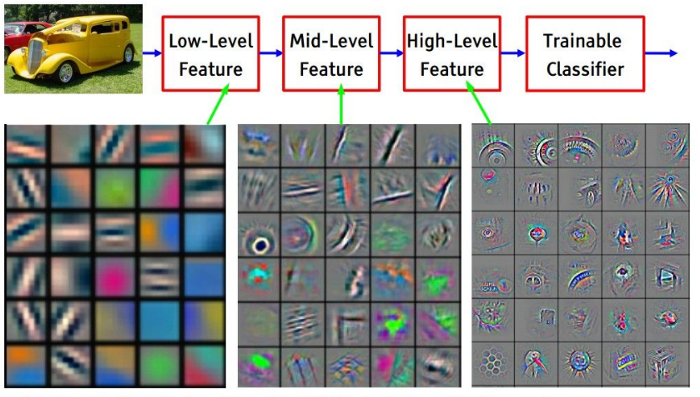
\includegraphics[width=\linewidth]{Images/ML/CNN_features.png}
    \caption{Feature-finding at increasing size scales, from~\cite{CNN_features}.}
    \label{fig:CNN_features}
\end{figure}

This type of architecture has several advantages over a simple DNN. For one, the CNN's successive feature finding makes it more robust than a DNN. Since a DNN must analyze an entire input image at once, it may end up learning how to recognize an object in a particular situation, but e.g. might not recognize the object when it is standing in front of a different background. On the other hand, since the CNN learns to recognize simple lines and shapes first, and then learns to recognize how they come together to form objects, these nets are less susceptible to irrelevant details in the image.

Furthermore, the CNN has far fewer trainable parameters than an equivalently sized DNN. Since we are only looking at small sections of the image at a time, we could have e.g. a 3x3 window sliding around on the image, which ends up containing only 10 trainable parameters (including a bias value). Typically for a single CNN layer we may have about 100 or so different filter windows, but the number of weights for all of these windows combined is still much smaller than what we would typically if we had used a dense neural layer.

\section{GoogLeNet}

Over the years there have been many improvements in image classification nets, often created in the context of competitions such as the ImageNet Recognition Challenge. One particular competition winner, GoogLeNet, introduced a couple of ideas which are still widely used in state-of-the-art image recognition nets today.

In particular, GoogLeNet introduced the idea of Inception modules (Figure~\ref{fig:inception}), which are able to combine feature information from multiple scales on the same layer. The Inception modules also introduced some training tricks which are able to vastly decrease the number of trainable connections in a deep net.

\begin{figure}[htbp]
    \centering
    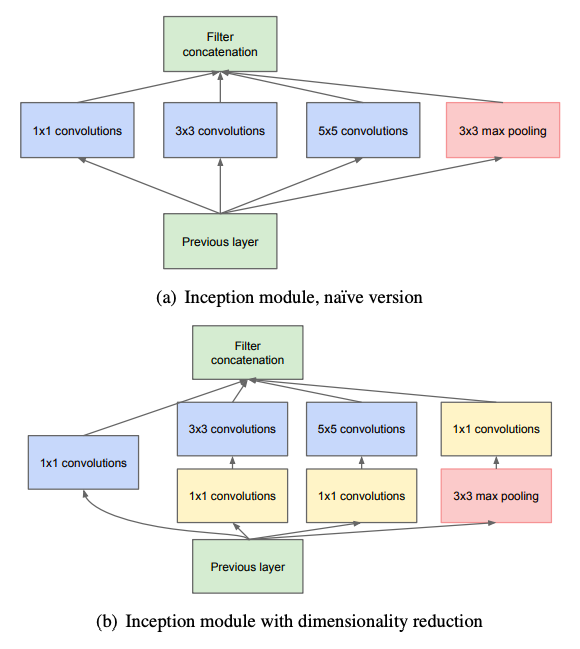
\includegraphics[width=0.7\linewidth]{Images/ML/inception.png}
    \caption{Inception module architecture, taken from~\cite{GoogLeNet}.}
    \label{fig:inception}
\end{figure}

These Inception modules are able to keep training parameters reduced to a reasonable number through the use of 1x1 dimensionality-reducing convolution layers. For example, if the output of our previous layer was a set of 256 feature maps, each of size 32x32, then our 1x1 layer may be a sliding window of size 1x1x256x64, which brings the number of filter maps down to 64 (still each of size 32x32). Performing this operation before 3x3 and 5x5 filters is especially useful for keeping the number of trainable parameters low.

The GoogLeNet architecture also included intermediate loss function terms, so that weights in the middle of the net could be more effectively trained. However, the authors of the GoogLeNet paper stated that these intermediate terms were later found to have only about $.5\%$ effect on classification accuracy.

\section{Autoencoders}

An autoencoder, shown in Figure~\ref{fig:autoencoder}, is an architecture which has the same number of neurons in its input and output layers, but which contains at least one hidden layer which has fewer neurons. These nets are trained in a semi-unsupervised manner, by simply trying to get the outputs to replicate the inputs. If we take $\hat{x}$ to be the input vector and $\hat{y}$ to be the output vector, a simple loss function for training an autoencoder is:

\begin{align}
    \mathcal{L} &= (\hat{y}-\hat{x})^2
\end{align}

\begin{figure}[htbp]
    \centering
    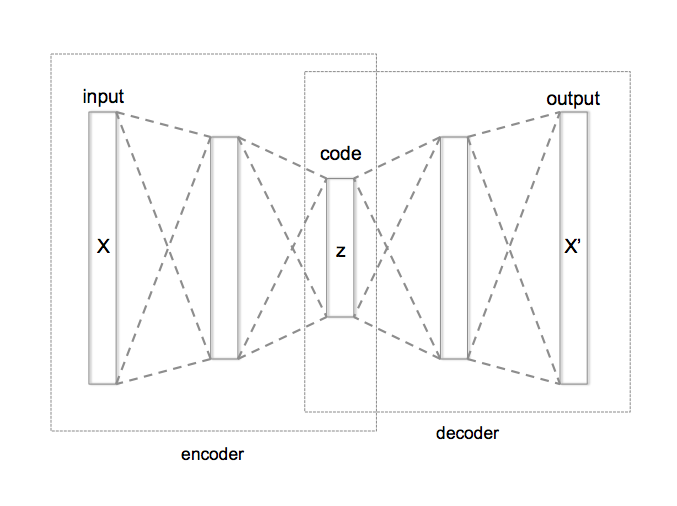
\includegraphics[width=\linewidth]{Images/ML/autoencoder.png}
    \caption{Autoencoder architecture, from~\cite{autoencoderDiagram}.}
    \label{fig:autoencoder}
\end{figure}

The purpose of an autoencoder is to perform dimensionality reduction. In Figure~\ref{fig:autoencoder}, our net has learned a compressed encoding of its data space, as represented by the neurons on the $\hat{z}$ layer. The trained structure can then be used for many purposes, such as for data compression or for image generation with generative adversarial nets.

The layers of the autoencoder may be simply connected, or they can be more complex structures, such as convolutional layers.

\section{Generative Adversarial Nets}

A generative adversarial network (GAN) can be used to create simulated samples in some data space. A GAN can be used to generate images, speech, video, or any other kind of data. Two famous examples of this type of network are StyleGAN, which can be used to generate faces and other images, and Google DeepDream, which can be used to generate surreal pictures and videos.

In a GAN we have two nets, the generator and the discriminator, competing against each other. To explain the process we will consider the case of a GAN which can generate images of a requested class.

The generator begins as the decoder half of a trained autoencoder, as seen in Figure~\ref{fig:autoencoder}. This autoencoder has been trained not only to replicate input data, but also to perform classification on it, as represented by a subset of the neurons on the $\hat{z}$ layer. Thus, layer $\hat{z}$ is a compressed representation of the image space, with a subset of neurons indicating image class and the rest of the neurons representing other salient features about the image.

In order to generate a new image with the generator, we feed to layer $\hat{z}$ the desired classification, along with a vector of randomized noise for the other neurons. Propagating through the generator creates an output of the desired class.

The discriminator half of the network is a trained classifier which is able to determine the class of an image. We tweak this architecture by adding an output which also classifies the image as "real" or "generated".

This is where the "adversarial" part of a GAN comes into play. The two nets are now trained against each other. First we request an image of a random class from the generator, and feed that image to the discriminator. The generator loss function is based on the image classification accuracy of the discriminator and on whether or not the discriminator was fooled into thinking the image was real. Next we train the discriminator by feeding it a mix of real and generated images, and grading it by discrimination accuracy. This process is repeated back and forth until convergence.

\section{Recurrent Neural Nets}

Up until now we have described typical feedforward neural nets, where connections between nodes go from layer to layer and do not loop back to previous layers. We will now describe a class of recurrent architectures which do not exhibit this behavior. Rather, as seen in Figure~\ref{fig:RNN}, a recurrent neural net (RNN) has a set of "hidden" neurons which loop from the output layer back to the input layer. We can use these kinds of nets for processing time series or sequential data by feeding the data sequence (e.g. a string of words that form a sentence) into the net one piece at a time. We begin with a randomly initialized hidden state. After each piece of input passes through the net, we get an output and an updated hidden state. The hidden state is brought back around to the beginning of the net, and is fed back in along with the next piece of sequential data. In this way the hidden neurons are able to act as a sort of memory state, and to encode some sort of ongoing information about the sequence. A recurrent net can turn a sequence of inputs into a sequence of outputs, but in many situations we only care about the final output, which may be used for classification.

\begin{figure}[htbp]
    \centering
    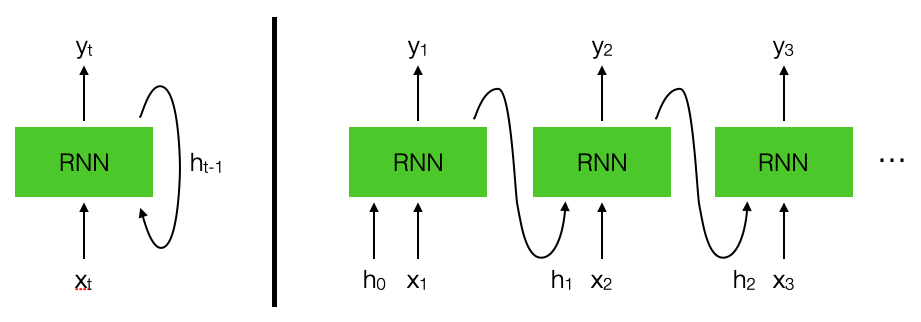
\includegraphics[width=\linewidth]{Images/ML/RNN.png}
    \caption{A standard recurrent neural net, shown in condensed form on the left, and in expanded form on the right. This net takes inputs $x_i$ and provides outputs $y_i$. A hidden state $h_i$ is retained in the net and passed back to the beginning after each input step.}
    \label{fig:RNN}
\end{figure}

The actual body of the RNN can be a neural net of any architecture, but in a standard RNN we typically use a simple few-layer densely connected net. The hidden state and output also typically pass through a $\tanh$ layer, with the output passing through an additional softmax layer. In this case, if we write the concatenation of $x_t$ and $h_{t-1}$ as $x_t \oplus h_{t-1}$ and the neural net weight matrix as $W$, we can represent the RNN via the following equations:

\begin{align}
    o_t\oplus h_t&=\tanh(W(x_t\oplus h_{t-1})) \\
    y_t&=\text{softmax}(o_t)
\end{align}

If we examine this equation, we can see a problem which commonly comes up when training an RNN via gradient descent. We see that the final output $y_n$ depends on $W$, $x_n$, and $h_{n-1}$. But then $h_{n-1}$ further depends on $x_{n-1}$ and $h_{n-2}$, and so on. If we work out the full derivative of $y_n$ with respect to $W$, we get the following:

\begin{align}
    \frac{dy_n}{dW}&=\frac{\partial y_n}{\partial W} + \frac{\partial y_n}{\partial h_{n-1}}\frac{dh_{n-1}}{dW} \\
    &=\frac{\partial y_n}{\partial W} + \frac{\partial y_n}{\partial h_{n-1}}[\frac{\partial h_{n-1}}{\partial W} + \frac{\partial h_{n-1}}{\partial h_{n-2}}\frac{dh_{n-2}}{dW}] \\
    &=\frac{\partial y_n}{\partial W} + \frac{\partial y_n}{\partial h_{n-1}}[\frac{\partial h_{n-1}}{\partial W} + \frac{\partial h_{n-1}}{\partial h_{n-2}}[
    \frac{\partial h_{n-2}}{\partial W} + \frac{\partial h_{n-2}}{\partial h_{n-3}}\frac{dh_{n-3}}{dW}
    ]] \\
    &=... \nonumber
\end{align}

We then see that for all $t$:

\begin{align}
    \frac{\partial h_t}{\partial h_{t-1}} &= \tanh'(W(x_t\oplus h_{t-1}))W \\
    \frac{\partial h_t}{\partial W} &= \tanh'(W(x_t\oplus h_{t-1}))(x_t\oplus h_{t-1}) \\
    \frac{dy_n}{dW} &\approx \sum_{t=1}^{n} [\tanh'(W(x_t\oplus h_{t-1}))]^{n+1-t}W^{n-t}(x_t\oplus h_{t-1})
\end{align}

The powers of $W$ and the powers of the derivative of $\tanh(x)$ are both problematic here, since they quickly approach zero, causing terms with low values of $t$ to essentially become irrelevant to training. In other words, the basic RNN has trouble learning long-range dependencies, and will in a sense "forget" the beginning of a sequence by the time it has calculated the final output. This behavior is called the vanishing gradient problem. In the case that W is large enough, we have the exploding gradient problem instead, but this issue is less common and is easily fixed by clipping gradients at a set maximum.

\section{LSTM and GRU}

One method of dealing with the vanishing gradient problem is the use of long short-term memory (LSTM) nets, first proposed in 1997. This type of net, shown in Figure~\ref{fig:LSTM_diagram}, has an internal structure in each recurrent cell which is more complex than a simple neural net. Each cell contains a forget gate, an input gate, and an output gate, which determine how much the cell state should update to accommodate new information, and how much information it should output. We have two internal states in an LSTM, $c_t$ and $h_t$. $c_t$ is similar to the hidden cell state in the basic RNN, and $h_t$ acts as the cell output at each step, but is also carried over to the input of the next step.

\begin{figure}[htbp]
    \centering
    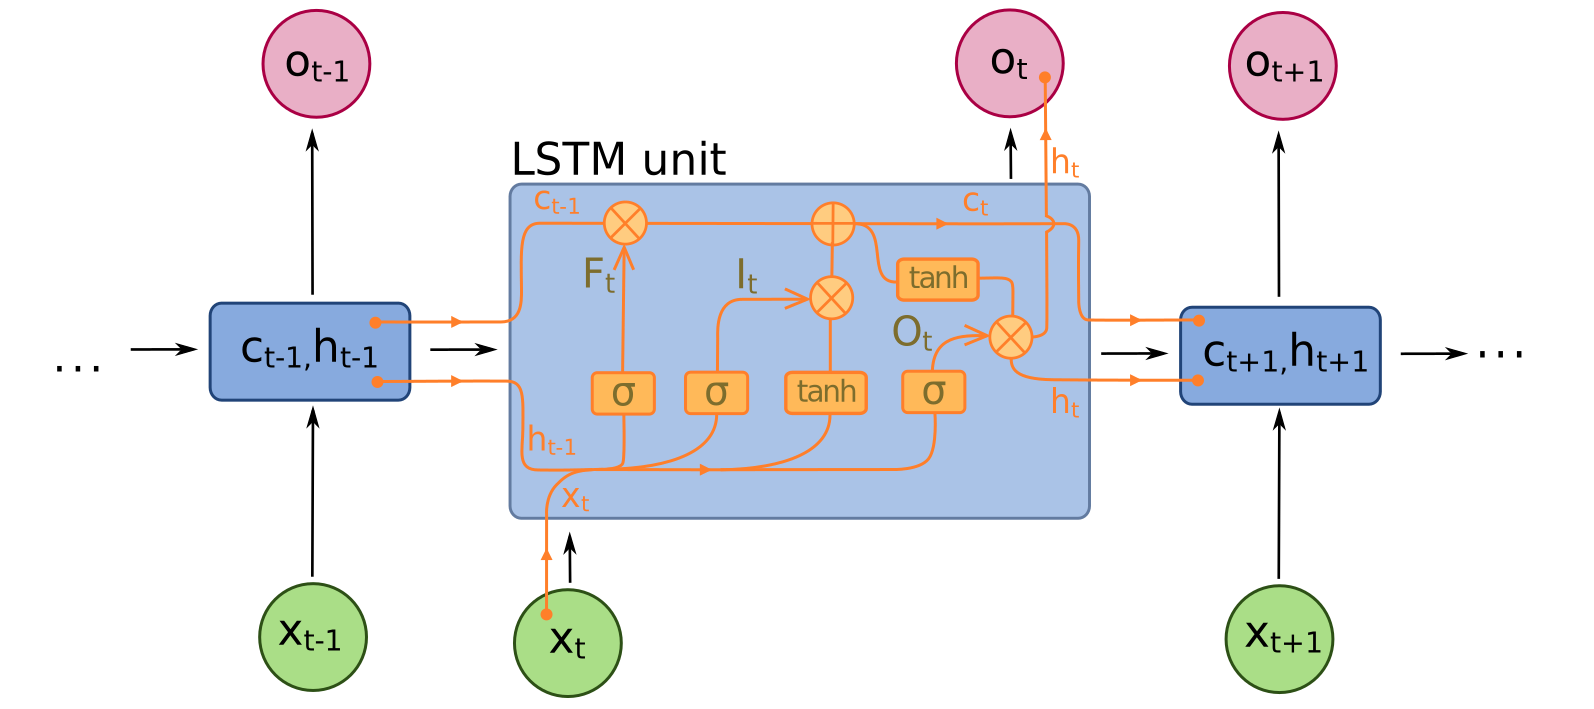
\includegraphics[width=\linewidth]{Images/ML/LSTM.png}
    \caption{LSTM architecture, showing the forget gate ($F_t$), input gate ($I_t$), and output gate ($O_t$) present in each cell. Taken from~\cite{LSTMDiagram}.}
    \label{fig:LSTM_diagram}
\end{figure}

The LSTM works as follows. At each time step $t$, we feed the input $x_t$, the previous output $h_{t-1}$, and the previous cell state $c_{t-1}$ into the net. $x_t$ and $h_{t-1}$ are used to determine the forget factor $F_t$, the input factor $I_t$, and the output factor $O_t$, all of which are vectors with components that lie between 0 and 1. The forget factor is multiplied onto $c_{t-1}$, allowing the cell to "forget" some of its previous state. The input factor is used to determine how much of the current input then gets added to the cell state. Finally, the output factor is multiplied by the new cell state to give $h_t$, the cell output. All together, the equations for an LSTM are as follows:

\begin{align}
    F_t &= \sigma(W_f (x_t \oplus h_{t-1})) \\
    I_t &= \sigma(W_i (x_t \oplus h_{t-1})) \\
    c_t &= c_{t-1} \cdot F_t + I_t \cdot\tanh(W_c (x_t \oplus h_{t-1})) \\
    O_t &= \sigma(W_o (x_t \oplus h_{t-1})) \\
    h_t &= O_t \cdot\tanh(W_h c_t)
\end{align}

The derivation is beyond the scope of this overview, but the gradient of the loss in this case will not have an exponential dependence on any weight matrix $W$, nor on the derivative of the sigmoid or tanh. Essentially, the $c_t$ state ensures that all inputs have non-zero contribution to the loss term. Thus, the LSTM is much less prone to the vanishing gradient problem.

The gated recurrent unit (GRU) net, introduced in 2014 and shown in Figure~\ref{fig:GRU_diagram}, further improves on the LSTM by reducing its complexity while maintaining its avoidance of the vanishing gradient problem. A GRU only has two gates, an update gate and a reset gate. In this architecture the reset gate controls how much information from the hidden state gets added to the input. The update gate conversely controls how much input information gets mixed back into the hidden state. The hidden state $h_t$ also acts as the output at each step, making the structure of the GRU somewhat less effective for multi-output data.

\begin{figure}[htbp]
    \centering
    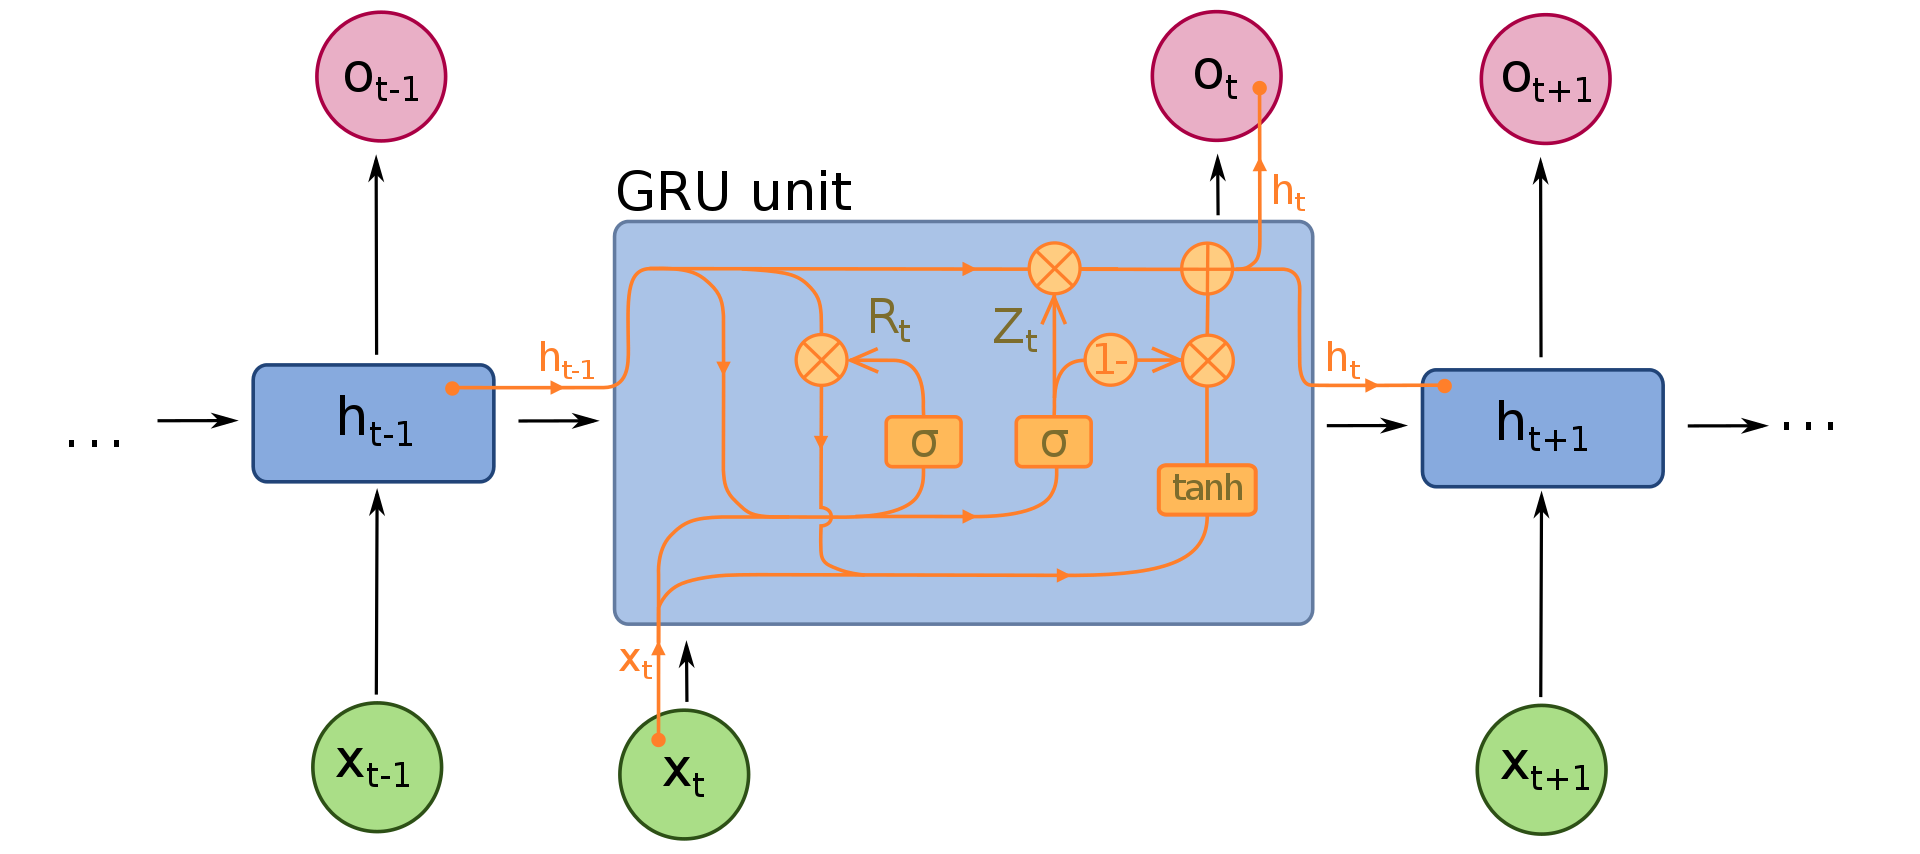
\includegraphics[width=\linewidth]{Images/ML/GRU.png}
    \caption{GRU architecture, showing the update gate ($Z_t$) and reset gate ($R_t$) present in each cell. Taken from~\cite{GRUDiagram}.}
    \label{fig:GRU_diagram}
\end{figure}

\begin{align}
    R_t &= \sigma(W_r (x_t \oplus h_{t-1})) \\
    Z_t &= \sigma(W_z (x_t \oplus h_{t-1})) \\
    h_t &= Z_t h_{t-1} + (1-Z_t)\tanh(R_t h_{t-1} + x_t)
\end{align}

\section{Seq2Seq}

A seq2seq architecture consists of an encoder recurrent net and a decoder recurrent net, as seen in Figure~\ref{fig:seq2seq}. This type of net takes an input sequence and processes it with the encoder. This processed vector, which contains information about the entire sequence, is then passed to the decoder and used to output a different sequence, not necessarily of the same length as the input.

\begin{figure}[htbp]
    \centering
    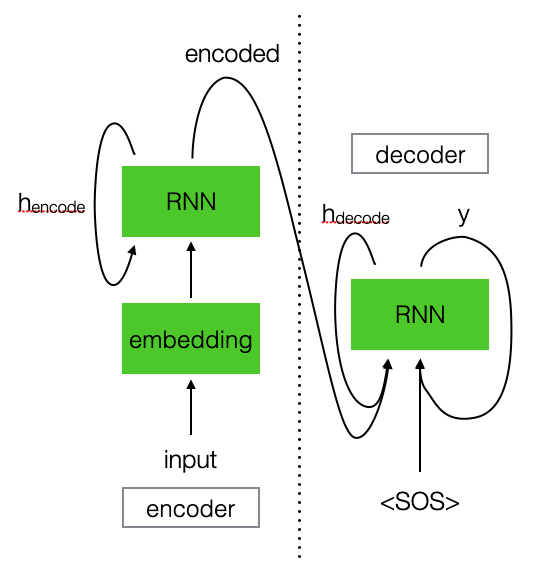
\includegraphics[width=0.55\linewidth]{Images/ML/seq2seq.png}
    \caption{Seq2Seq architecture. The encoder takes words in a sentence, embeds them in a word vector space, and passes the embedded vectors into an RNN. The final output of the encoder is sent to the decoder as its initial hidden state. The decoder begins with SOS as its initial input, and loops until it outputs EOS. The entire decoder sequence is the output sentence.}
    \label{fig:seq2seq}
\end{figure}

Seq2Seq is commonly used for language translation, so inputs in these cases are first transformed into a "word vector" in some embedding space before they go through the encoder. Describing word embeddings is outside the scope of this review, but the idea is that similar words are close together in this vector space, and pairs of words with the same relations have similar vector differences. In other words, the embedding captures some semantic structure between words. Common embeddings include word2vec and GloVe.

In more detail, the encoder takes a sequence of inputs $\hat{x}$ and runs it through an RNN to produce a sequence of outputs $\hat{s}$. In a simple seq2seq architecture, we take only the final output, which we denote as $s$, to pass to the decoder. The decoder takes $s$ as an initial hidden state, and the start-of-string (SOS) signal as an initial input, and performs a typical recurrent architecture loop to generate an output sequence. The sequence ends when the decoder outputs an end-of-string (EOS) signal.

A seq2seq architecture may also include an attention mechanism, as shown in Figure~\ref{fig:seq2seq_with_attention}. In this case the decoder has an additional step where it uses its input and hidden state to obtain an attention vector. We take the dot product of this attention vector with the entire encoder output sequence $\hat{s}$ to get a sort of weighted vector. Essentially, the attention vector allows us to focus on different parts of the input sequence as we're producing the output.

Details about the training of seq2seq are outside the scope of this review.

\begin{figure}[htbp]
    \centering
    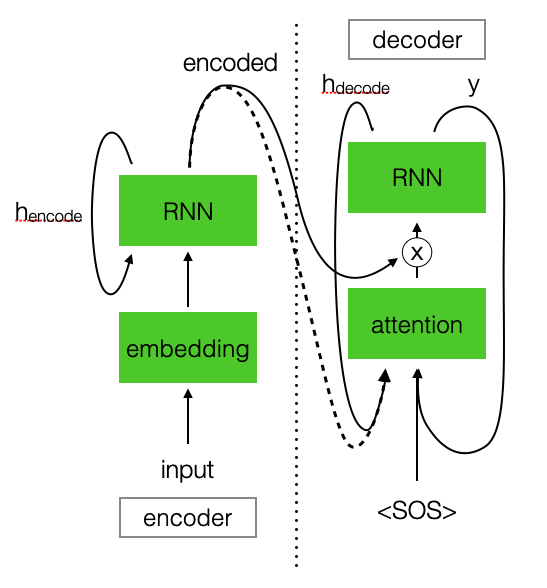
\includegraphics[width=0.55\linewidth]{Images/ML/seq2seq_with_attention.png}
    \caption{Seq2Seq architecture with an attention mechanism added. Now the entire encoder output is used by the decoder. The final output of the encoder is still used as the decoder's initial hidden state, but now the hidden state and decoder input are used to calculate an attention vector, which passes through a softmax layer to add up to 1. The dot product of this attention vector with the entire encoder output sequence then produces a weighted encoder output which is sent to the decoder RNN.}
    \label{fig:seq2seq_with_attention}
\end{figure}

\section{Transformers}

Transformers build on the idea of using attention, but take the concept further by removing the recurrent neural net from the encoder altogether and relying solely on attention to encode positional and relational information~\cite{transformer}. The transformer thus relies on attention to figure out which parts of the input are important for the decoder at each step of the output.

The transformer architecture is shown in Figure~\ref{fig:transformer}. Once again the input is embedded in some word space before being fed to the encoder. However, now we also add an additional positional encoding vector onto each word to represent its location in the input sequence, to make up for the lack of an RNN. A detailed description of the positional encoding is beyond the scope of this review. The encoder itself is then made up of a series of sequential modules each composed of a multi-head attention mechanism (described below) and a feedforward net. A skip connection is used to add the input of each sublayer to its output.

\begin{figure}[htbp]
    \centering
    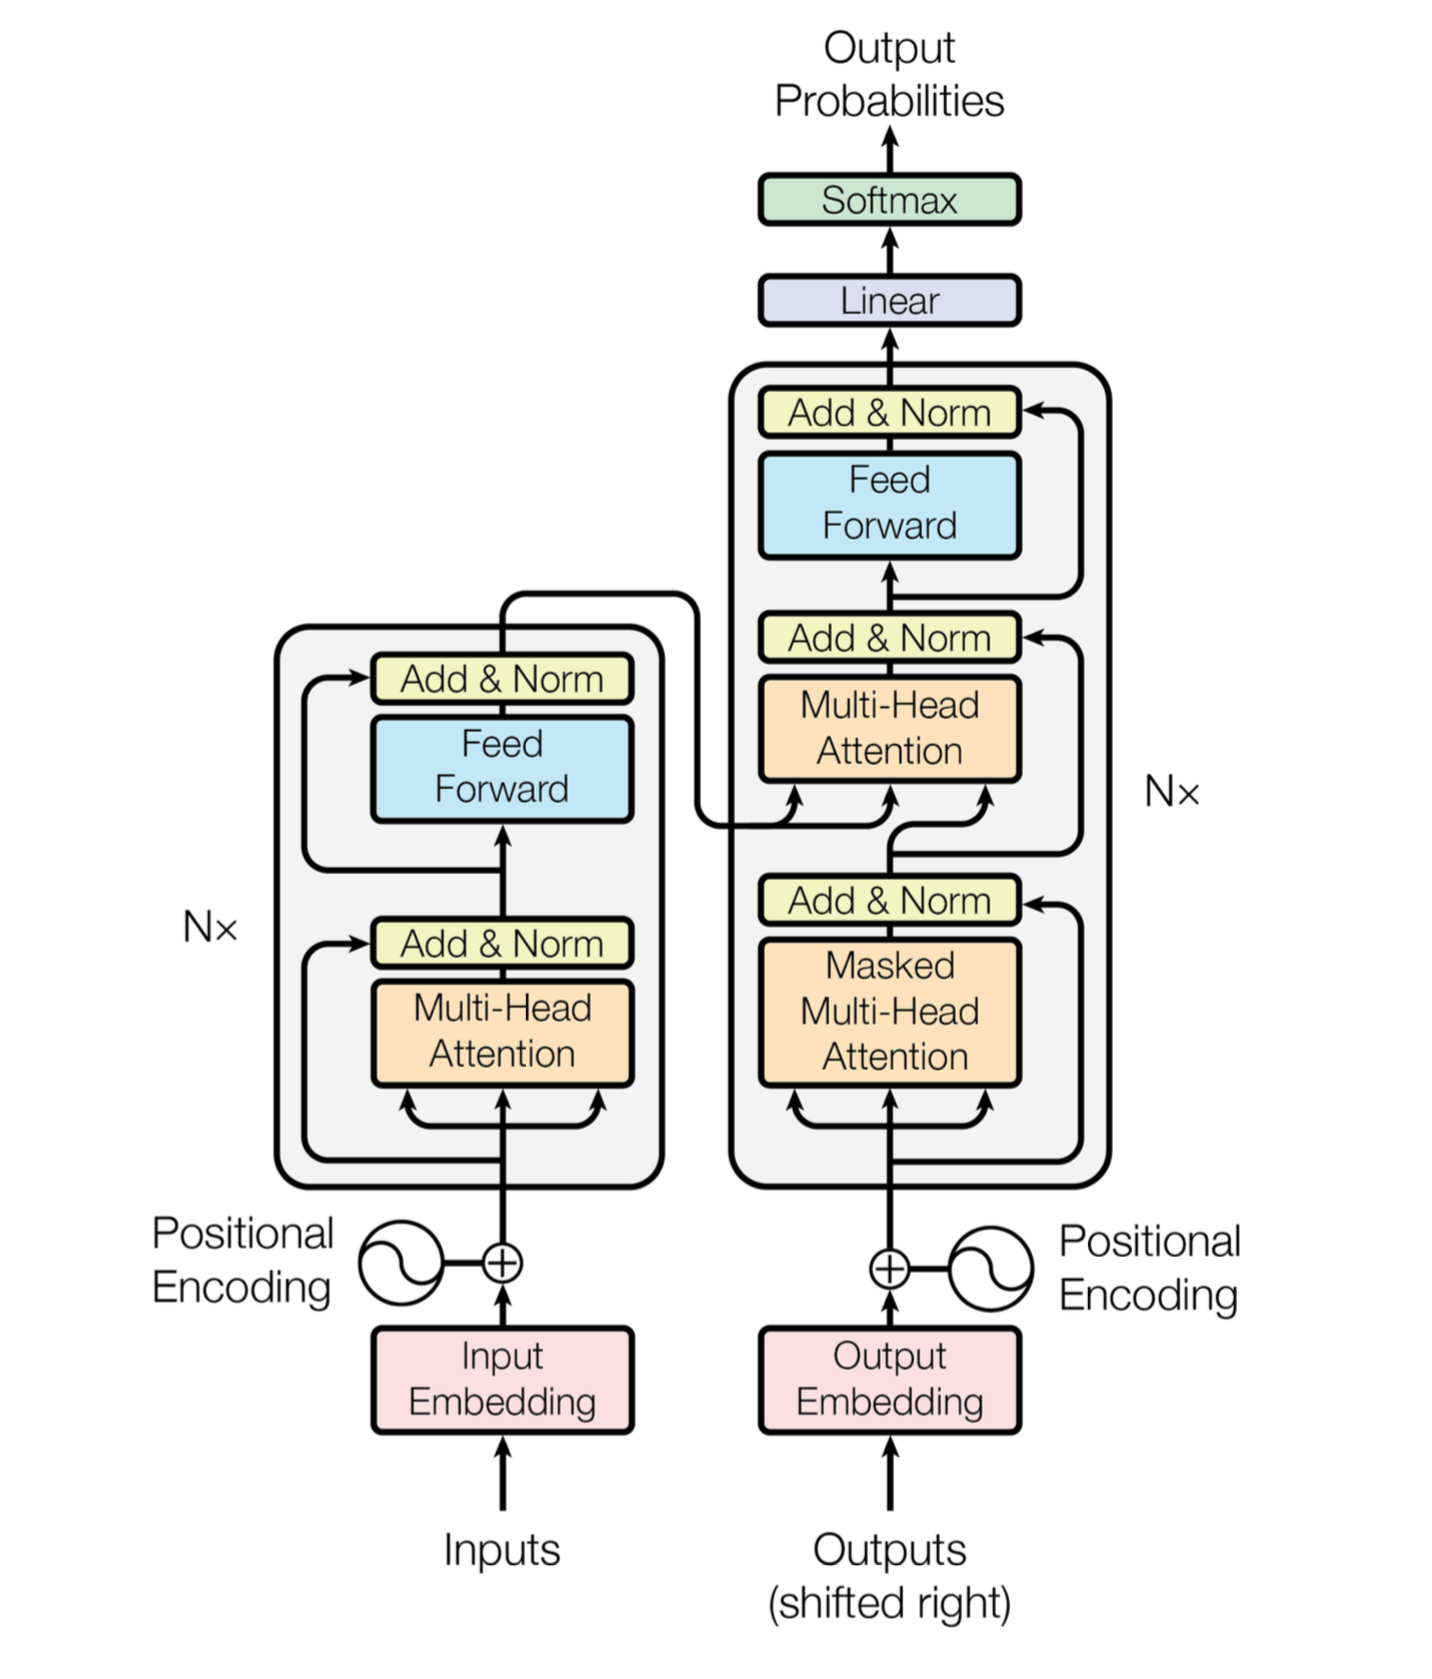
\includegraphics[width=0.7\linewidth]{Images/ML/transformer.png}
    \caption{Transformer architecture. Taken from~\cite{transformer}.}
    \label{fig:transformer}
\end{figure}

The multi-head attention mechanism in shown in Figure~\ref{fig:transformer_dot_product_attention}. Here, $Q$, $K$, and $V$ stand for query, key, and value. The $Q$ and $K$ vectors are used as in a content retrieval system, where the dot product of two vectors indicates their similarity. $V$ is the representation of a word in whatever relevant space we're using, and may or may not be equivalent to $K$. $Q$ and $K$ are of dimension $d_k$, and $V$ is of dimension $d_v$. In the simplest example, the vector embeddings of the input words are used for $Q$, $K$, and $V$, with all three matrices being equivalent. Using each word in an input this way to calculate an attention vector for the other words in the input is a concept called self-attention. The total self-attention matrix is then calculated as follows, where we have used a scaling factor to normalize the matrix product:

\begin{align}
    Attention(Q,K,V)&=\text{softmax}(\frac{QK^T}{\sqrt{d_k}})V
\end{align}

\begin{figure}[htbp]
    \centering
    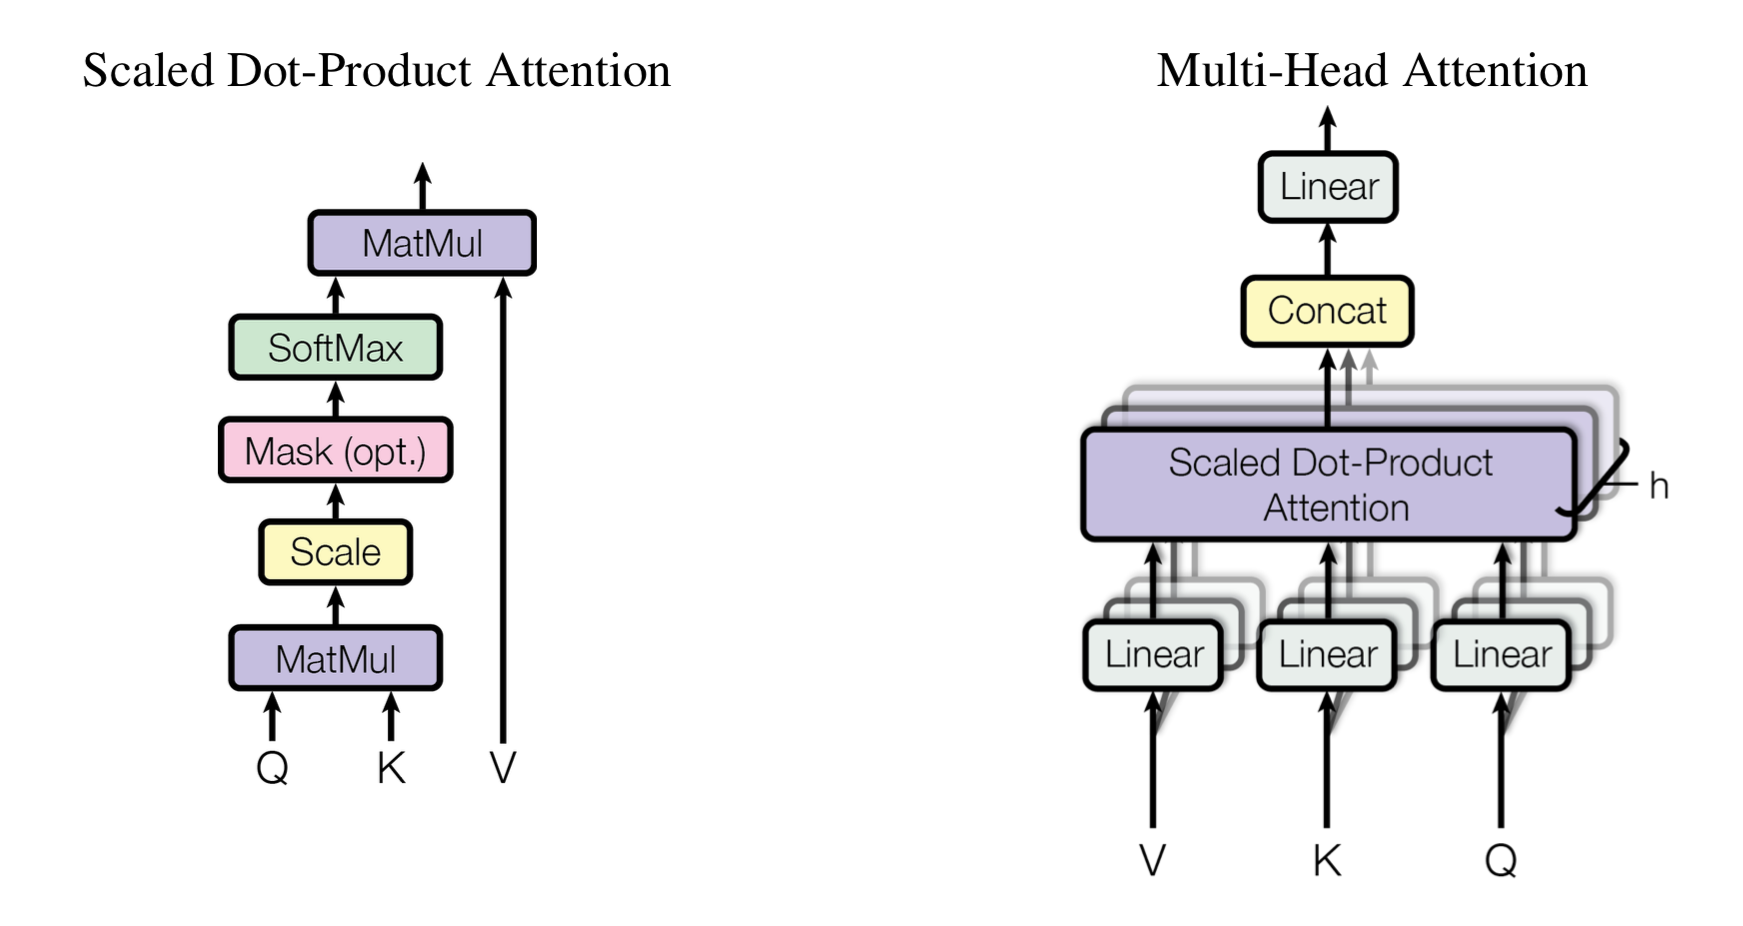
\includegraphics[width=\linewidth]{Images/ML/transformer_dot_product_attention.png}
    \caption{Mutli-head self attention mechanism. Taken from~\cite{transformer}.}
    \label{fig:transformer_dot_product_attention}
\end{figure}

In a more general multi-head attention mechanism, we don't simply use the word vector embeddings for $Q$, $K$, and $V$. Rather, we learn $h$ different sets of vectors $v_Q$, $v_K$, and $v_V$, which we project our word embeddings upon in order to obtain $h$ sets of $Q$, $K$, and $V$. The end result is that we get $h$ sets of attention matrices, where each attention matrix is some attention-weighted encoding of the relevant self-context for each input word. The $h$ matrices are then concatenated and sent through a linear layer to provide a single input-sequence encoding.

The decoder uses the same multi-headed attention idea, but the attention layer is masked, so that during training the decoder can only see words which have been outputted so far, rather than the entire output sequence. There is also a second multi-headed attention layer, which uses the output of the encoder for the keys and values.

\section{Deep Sets}

\section {Set Transformers}